\documentclass[11pt]{article}

\usepackage[margin=1in]{geometry}
\usepackage{graphicx}
\usepackage{hyperref}
\usepackage{setspace}
\doublespacing

\begin{document}
\title{Quantitative Formal Methods\\Modelling Speedoo}
\author{Renan Greca}
\maketitle

\section*{Introduction}
Speedoo, introduced by Chen et al. \cite{speedoo2018}, is a tool designed to help software developers find optimization opportunities in large-scale programs.
Instead of just outputting a list of methods that should be optimized, the core of the Speedooo solution lies on the concept of \textit{optimization spaces}, each of which is a set of related methods that together provide one optimization opportunity.

For example, if two methods $f$ and $g$ are reasonably fast in isolation, a traditional tool might not suggest them as optimization opportunities.
However, if $f$ calls $g$ multiple times during execution, $f$ and $g$ form an optimization space and should be analyzed by the developers together -- perhaps there is a way of optimizing the number of calls to $g$ within $f$.

This document describes the process of modelling Speedoo using a petri net, which provides some insight regarding the running times of the steps taken by an execution of Speedoo.
Furthermore, it also provides a comparison with another optimization-suggesting tool, YourKit, using discrete-time markov chains.

\section*{Modelling Speedoo's petri net}
To analyze Speedoo, a petri net was designed using the PIPE tool \cite{pipe2002}.
The steps taken by the tool were used as a general guide of the places and transitions of the network.
Figure 2 from the Speedoo article provides the steps, complemented by Table 8, also from Speedoo, which provides the performance overhead of each step.

The most relevant step for this analysis is the first one, entitled Metric Computation.
For Speedoo, the authors use three separate tools: 
\begin{enumerate}
	\item Titan, which computes \textit{Architectural Metrics} (AM);
	\item Understand, which computes \textit{Static Complexity Metrics} (SCM); and
	\item YourKit, which computes \textit{Dynamic Execution Metrics} (DEM).
\end{enumerate}
Here, we assume the there tools run in parallel, so their computations are modelled as such in the petri net.

Furthermore, the Speedoo article provides the time each tool takes to compute metrics, and these times were used to assign rates to the petri net transitions.
Speedoo was tested on three separate projects, so the average time was taken for each computation (we can interpret this as ``average running time for a project of arbitrary size'').
Then, these times were normalized and subtracted from 1, so longer times approach 1 and shorter times approach 0.
A simple algorithm was developed to quickly retrieve these values.

The other two major steps of Speedoo, Method Priotization and Optimization Space Localization, were each modelled as a single step, for two reasons:
first, their sub-steps are dependent of each other, so they must be executed linearly and cannot take advantage of parallelism;
and second, the paper only provides the total running time of these steps.

\begin{figure*}[!htbp]
\centering
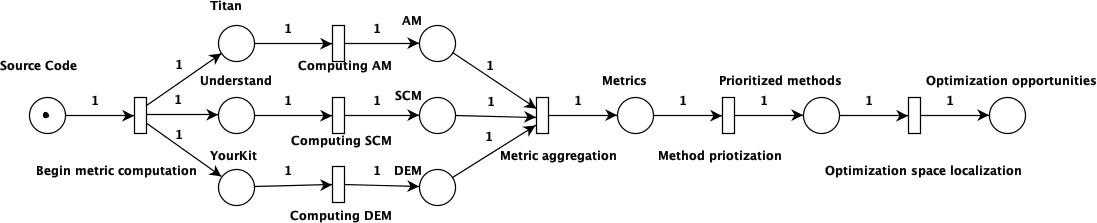
\includegraphics[scale=0.4]{speedoo_petrinet.png}
\caption{The petri net describing Speedoo}
\label{fig:petrinet}
\end{figure*}

Figure \autoref{fig:petrinet} shows the petri net that describes the steps taken by Speedoo.
An execution of the petri net is as follows:
\begin{enumerate}
	\item Speedoo starts at an initial place which contains the input project's source code;
	\item Then, this source code is duplicated and sent to the three tools for metric computation;
	\item Each tool computes the appropriate metric;
	\item Once all metrics are computed, they are sent back to Speedoo;
	\item With the computed metrics, the Method Priotization step is performed;
	\item With the prioritized methods, the Optimization Space Localization step is performed, producing the desired output.
\end{enumerate}

With this, we can run analysis on the petri net and find out some information about it.
\autoref{table:states} shows the reachable states of the petri nets: each column is a place and each row is a state in which places have a certain number of tokens.
We can see that, due to the parallel computation of metrics, states M1 through M8 represent all the possible permutations of metrics being computed, depending on which tools performs its analysis faster.

\begin{table}[]
\centering
\begin{tabular}{l|c|c|c|c|c|c|c|c|c|c|}
\textbf{}    & \textbf{\begin{tabular}[c]{@{}c@{}}Src.\\ code\end{tabular}} & \textbf{Titan} & \textbf{Under.} & \textbf{YourKit} & \textbf{AM} & \textbf{SCM} & \textbf{DEM} & \textbf{Metrics} & \textbf{\begin{tabular}[c]{@{}c@{}}Pr. \\ meth.\end{tabular}} & \textbf{\begin{tabular}[c]{@{}c@{}}Opt.\\ opp.\end{tabular}} \\ \hline
\textbf{M0}  & 1                                                            & 0              & 0               & 0                & 0           & 0            & 0            & 0                & 0                                                             & 0                                                            \\ \hline
\textbf{M1}  & 0                                                            & 1              & 1               & 1                & 0           & 0            & 0            & 0                & 0                                                             & 0                                                            \\ \hline
\textbf{M2}  & 0                                                            & 1              & 1               & 0                & 0           & 0            & 1            & 0                & 0                                                             & 0                                                            \\ \hline
\textbf{M3}  & 0                                                            & 1              & 0               & 1                & 0           & 1            & 0            & 0                & 0                                                             & 0                                                            \\ \hline
\textbf{M4}  & 0                                                            & 0              & 1               & 1                & 1           & 0            & 0            & 0                & 0                                                             & 0                                                            \\ \hline
\textbf{M5}  & 0                                                            & 1              & 0               & 0                & 0           & 1            & 1            & 0                & 0                                                             & 0                                                            \\ \hline
\textbf{M6}  & 0                                                            & 0              & 1               & 0                & 1           & 0            & 1            & 0                & 0                                                             & 0                                                            \\ \hline
\textbf{M7}  & 0                                                            & 0              & 0               & 1                & 1           & 1            & 0            & 0                & 0                                                             & 0                                                            \\ \hline
\textbf{M8}  & 0                                                            & 0              & 0               & 0                & 1           & 1            & 1            & 0                & 0                                                             & 0                                                            \\ \hline
\textbf{M9}  & 0                                                            & 0              & 0               & 0                & 0           & 0            & 0            & 1                & 0                                                             & 0                                                            \\ \hline
\textbf{M10} & 0                                                            & 0              & 0               & 0                & 0           & 0            & 0            & 0                & 1                                                             & 0                                                            \\ \hline
\textbf{M11} & 0                                                            & 0              & 0               & 0                & 0           & 0            & 0            & 0                & 0                                                             & 1                                                            \\ \hline
\end{tabular}
\caption{The reachable states of the petri net}
\label{table:states}
\end{table}

However, despite all these states being reachable, they are not equally likely.
This happens because the Dynamic Execution Metrics take much longer to compute than the other metrics -- making it so step M7 is the one in which the model spends the most time.
Indeed, since the computation of Dynamic Execution Metrics takes hours instead of seconds, the time spent waiting for YourKit is several orders of magnitude greater than anything else in the model.

\begin{table}[]
\centering
\begin{tabular}{l|c|}
\multicolumn{1}{c|}{\textbf{State}} & \textbf{Value} \\ \hline
\textbf{M0}                         & 1              \\ \hline
\textbf{M1}                         & 0.50018        \\ \hline
\textbf{M2}                         & 0.5002         \\ \hline
\textbf{M3}                         & 0.9999         \\ \hline
\textbf{M4}                         & 1.0007         \\ \hline
\textbf{M5}                         & 1              \\ \hline
\textbf{M6}                         & 1.0008         \\ \hline
\textbf{M7}                         & 10,000         \\ \hline
\textbf{M8}                         & 1              \\ \hline
\textbf{M9}                         & 1.0002         \\ \hline
\textbf{M10}                        & 1.00432        \\ \hline
\textbf{M11}                        & $\infty$       \\ \hline
\end{tabular}
\caption{Time spent in each state of the petri net}
\label{table:times}
\end{table}

Due to the relative simplicity of the petri net model, not much else can be extracted from the analysis.
The program always terminates and produces an output, and there are no cyclic paths, so the time spent on M11, the final state, tends to infinity.
In this case, waiting longer for the Dynamic Execution Metrics is rather obvious from the data -- it's thousands of times slower than other operations.
However, if the times were more comparable, this analysis could be an interesting way of detecting bottlenecks in the process.

\section*{Modelling Speedoo's markov chain}

Another analysis of Speedoo was performed using discrete-time markov chains, which allow us to determine how many iterations it would take for a value to reach a steady state.
For the purposes of this work, we used information provided in Table 6 of the Speedoo article, which details the density of suggested methods that were actually optimized in the projects the authors considered.
To model and run the markov chains, the Octave tool was used \cite{octave1993}.

Here, we consider two such projects: Avro and PDFBox.
Assuming that, for every new release of a project, the same percentage of suggested methods are optimized, we want to find out how many releases it would take for all the suggested methods to be optimized.
Furthermore, we also assume that, once a method has been optimized, it is never suggested again.

In all figures, the red points represent the proportion of suggested methods that were optimized, while the blue points show the proportion of methods that still need to be optimized.

As such, \autoref{fig:speedoo-avro} shows that, using Speedoo, it would take around 50 releases for Avro to optimize all the methods suggested.
PDFBox, on the other hand, would take only 12, shown in \autoref{fig:speedoo-pdfbox}.

The alternative to Speedoo investigated by the authors, YourKit, proves much worse using the same criteria: Avro would take over 140 releases to be optimized (\autoref{fig:yourkit-avro}) while PDFBox would take nearly 40 releases (\autoref{fig:yourkit-pdfbox}).

However, in order to achieve these results, many assumptions about the projects had to be made.
Realistically, software optimization does not evolve at a constant pace and it cannot be expected that all methods are truly optimizable.

Therefore, although this analysis provides an interesting comparison between Speedoo and YourKit, it does not provide a concrete measure of Speedoo's efficacy.

\begin{figure*}[!htbp]
\centering
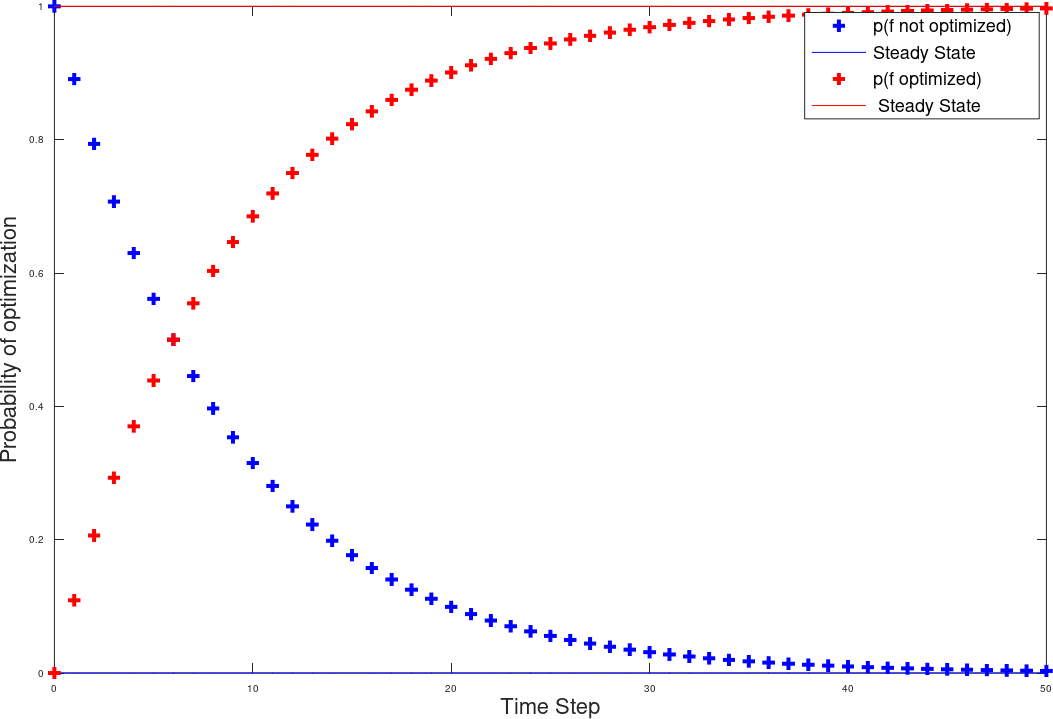
\includegraphics[scale=0.6]{speedoo-avro.png}
\caption{Running Speedoo on the Avro project}
\label{fig:speedoo-avro}
\end{figure*}

\begin{figure*}[!htbp]
\centering
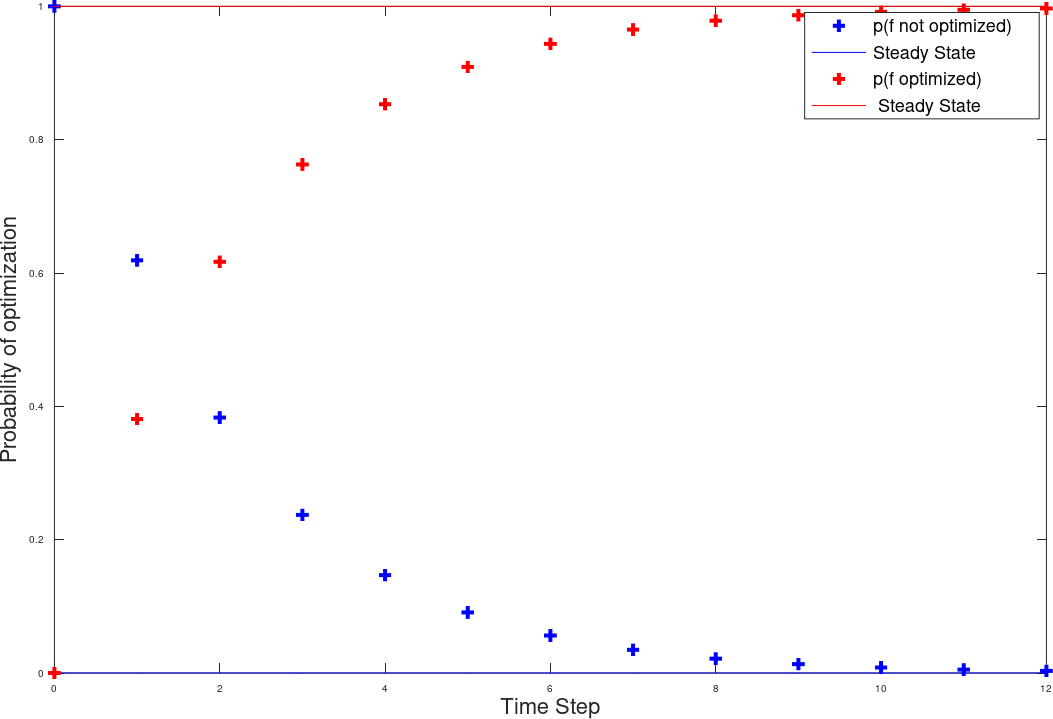
\includegraphics[scale=0.6]{speedoo-pdfbox.png}
\caption{Running Speedoo on the PDFBox project}
\label{fig:speedoo-pdfbox}
\end{figure*}

\begin{figure*}[!htbp]
\centering
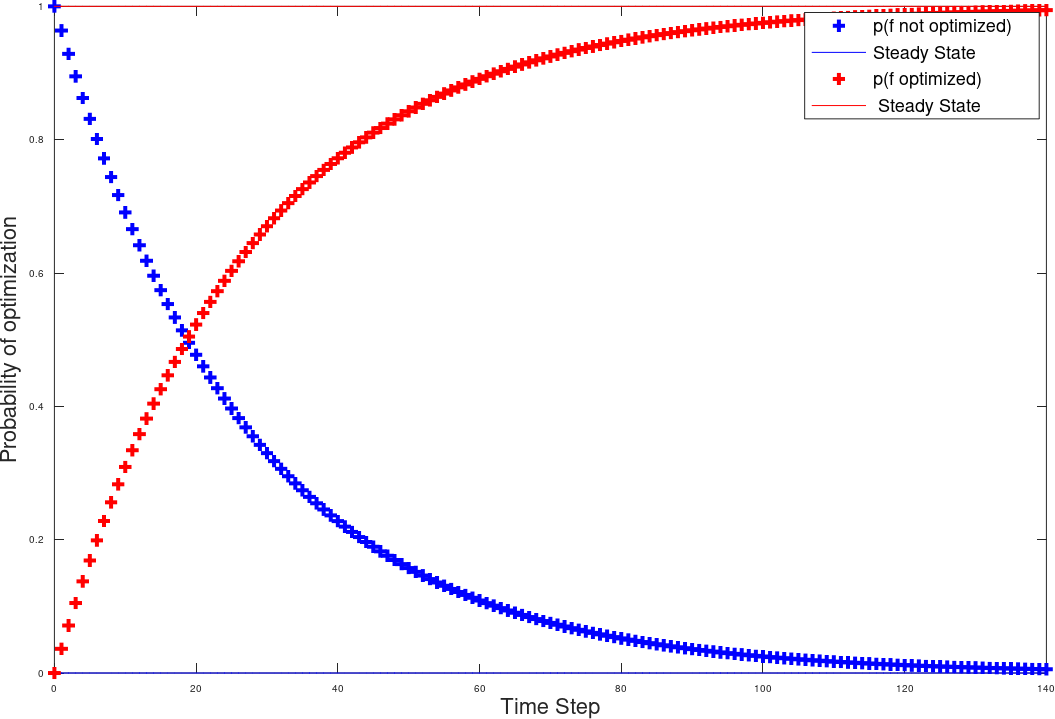
\includegraphics[scale=0.6]{yourkit-avro.png}
\caption{Running YourKit on the Avro project}
\label{fig:yourkit-avro}
\end{figure*}

\begin{figure*}[!htbp]
\centering
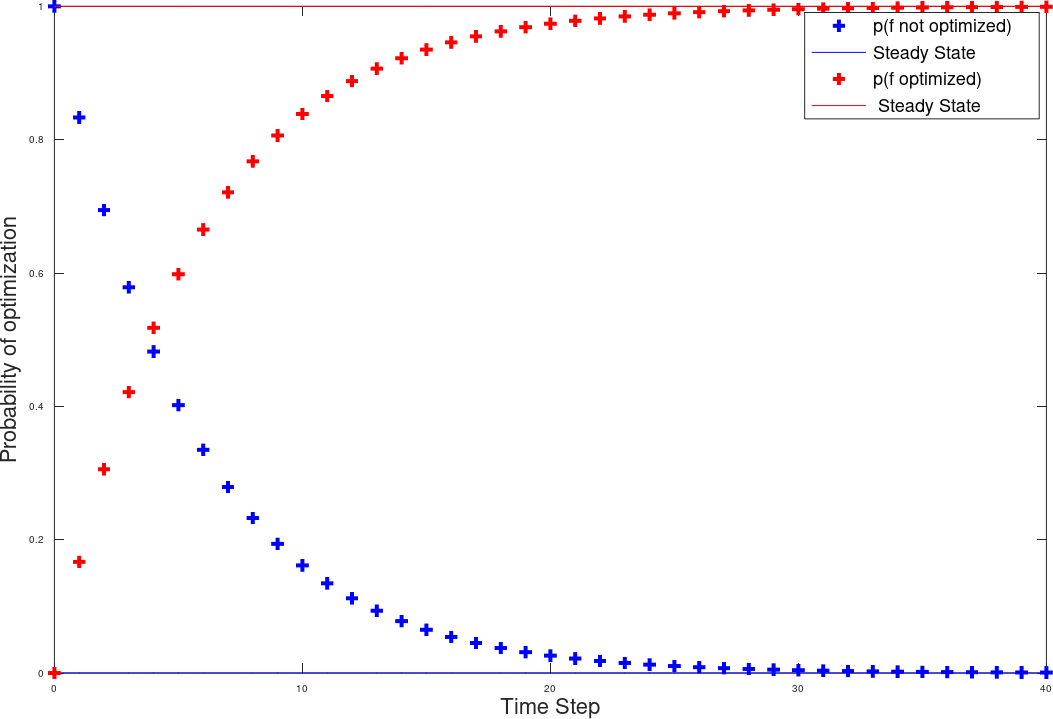
\includegraphics[scale=0.6]{yourkit-pdfbox.png}
\caption{Running YourKit on the PDFBox project}
\label{fig:yourkit-pdfbox}
\end{figure*}

\section*{Conclusion}

In this work, the Speedoo optimization tool was analysed by modelling its steps and results using a petri net and markov chains.

The petri net and the markov chains used here are just an interpretation of Speedoo, using information available on the article that presents the tool.
Other interpretations, possibly with different sets of information, could generate different representations and even different analyses of Speedoo.

The models introduced here succeed in providing us with two pieces of information:
first, the petri net clearly shows the bottleneck created by the Dynamic Execution Metrics computation;
and second, the markov chains show how much longer it would take to optimize a software project using Speedoo's alternative YourKit.

\begin{thebibliography}{99}
 
\bibitem{speedoo2018} Chen Z, Chen B, Xiao L, Wang X, Chen L, Liu Y, Xu B (2018), \textquotedblleft Speedoo: Prioritizing Performance Optimization Opportunities,\textquotedblright\ \textit{Proceedings of the 40th International Conference on Software Engineering  - ICSE '18}.

\bibitem{pipe2002} Department of Computing, Imperial College London (2002), \textquotedblleft The Platform Independent Petri net Editor PIPE,\textquotedblright\ \url{http://pipe2.sourceforge.net}.

\bibitem{octave1993} Eaton JW (1993), \textquotedblleft GNU Octave,\textquotedblright\ \url{https://www.gnu.org/software/octave/}.


\end{thebibliography}


\end{document}
